\documentclass[14pt]{extreport}

\usepackage[utf8]{inputenc}
\usepackage[T2A]{fontenc}
\usepackage[english,ukrainian]{babel}
\usepackage{tempora}

\usepackage{float}
\usepackage{caption}
\captionsetup[table]{justification=raggedleft, singlelinecheck=false, labelsep=period}
\captionsetup[figure]{labelsep=space}
\usepackage{graphicx}
\graphicspath{ {./pictures} }

\linespread{1.5}
\setlength{\parskip}{0pt}
\usepackage{indentfirst}

\usepackage[a4paper,top=20mm,bottom=20mm,left=25mm,right=10mm]{geometry}

\usepackage{fancyhdr}
\fancypagestyle{plain}{
  \pagestyle{myheadings}
}
\pagestyle{myheadings}
\setcounter{page}{4}

\setcounter{secnumdepth}{3}
\newcounter{req}[subsubsection]
\newcommand\req{\arabic{req}\stepcounter{req}}

\usepackage{titlesec}
\titleformat{\chapter}{\centering\bfseries\MakeUppercase}{\chaptername~\thechapter.}{1pc}{}
\titleformat{\section}{\bfseries}{\thesection.}{1pc}{}
\titleformat{\subsection}{\bfseries}{\thesubsection.}{1pc}{}
\titleformat{\subsubsection}{\bfseries}{\thesubsubsection.}{1pc}{}
% \titleformat{\paragraph}{\bfseries}{}{}{}

\titlespacing*{\chapter}{0pt}{10mm}{14pt}
\titlespacing*{\section}{\parindent}{14pt}{0pt}
\titlespacing*{\subsection}{\parindent}{0pt}{0pt}
\titlespacing*{\subsubsection}{\parindent}{0pt}{0pt}
\titlespacing*{\paragraph}{\parindent}{0pt}{7pt}

\usepackage{enumitem}
\setlist{nolistsep}

\usepackage{hyperref}
\def\UrlBreaks{\do\/\do-}

\begin{document}
  \chapter*{Анотація}
  
  \tableofcontents
  \newpage
  
  \chapter*{Вступ}
  \addcontentsline{toc}{chapter}{Вступ}
  
  У сучасному світі цифрові технології відіграють ключову роль у забезпеченні прозорості, достовірності та довіри в різних сферах суспільного життя. Однією з таких сфер є електронне голосування — інноваційний підхід до організації виборів, який дедалі частіше використовується як альтернатива традиційним паперовим методам. Електронне голосування дозволяє зменшити витрати часу та ресурсів, підвищити зручність участі, а також розширити коло учасників. Однак широке впровадження таких систем стикається з рядом викликів, серед яких — забезпечення цілісності даних, запобігання фальсифікаціям, гарантування конфіденційності виборців, а також підтвердження легітимності результатів.

  Сучасні централізовані електронні системи голосування залишаються вразливими до низки загроз, включно з технічними збоями, зовнішніми атаками, внутрішніми маніпуляціями та недовірою з боку користувачів. Відсутність повної прозорості процесу створює передумови для спотворення результатів, що у свою чергу знижує рівень довіри суспільства до інституцій, які організовують такі голосування. Одним із перспективних напрямів розв'язання цих проблем є використання технології блокчейн. Блокчейн знаходить застосування в багатьох галузях, включаючи фінанси, логістику, охорону здоров'я та управління ланцюгами поставок. У контексті електронного голосування він дозволяє забезпечити прозорість, конфіденційність і захищеність голосів: кожен голос у такій системі зберігається у вигляді транзакції, яка є незмінною та відкритою для перевірки всіма учасниками. Завдяки цьому досягається високий рівень довіри до процесу голосування навіть без централізованого контролю.

  Актуальність теми цієї роботи зумовлена потребою у створенні сучасних електронних систем голосування, які забезпечуватимуть високий рівень безпеки та довіри. З розвитком технологій все більше організацій, компаній та державних установ прагнуть впроваджувати цифрові рішення для голосування, що потребує детального аналізу існуючих підходів, а також розробки нових моделей, що враховуватимуть їх переваги та недоліки.

  Метою роботи є проектування системи для проведення голосувань та опитувань, яка відповідатиме вимогам прозорості, безпеки та достовірності результатів. Для забезпечення поставленої мети розроблено архітектуру системи голосування, яка відповідає вимогам безпеки, надійності та ефективності.

  Для досягнення поставленої мети необхідно виконати низку задач, зокрема провести комплексне дослідження існуючих рішень у сфері електронного голосування, зосередивши увагу на системах, побудованих із використанням технології блокчейн. На основі цього слід визначити ключові переваги та недоліки таких рішень і сформулювати вимоги до безпечної, прозорої та зручної у використанні платформи для голосування. Далі потрібно спроєктувати архітектуру майбутньої системи, що передбачає механізми створення голосувань, автентифікації користувачів, захисту даних і прозорої обробки результатів. Після цього необхідно реалізувати основні компоненти системи та провести тестування з метою перевірки її функціональності, стабільності роботи й відповідності визначеним вимогам безпеки.

  Результати цієї роботи можуть бути використані для подальшого розвитку електронних систем голосування, а також як основа для впровадження подібних рішень у різних сферах діяльності — від державного управління до корпоративних голосувань та соціальних опитувань.
  
  % Оглядовий розділ
  \chapter{Теоретичні основи та аналіз сучасних підходів до організації електронних голосувань}
  
  \section{Основи блокчейн-технології}

  Блокчейн є децентралізованою технологією зберігання даних, яка дозволяє створювати надійні розподілені системи, що виключають необхідність довіри до єдиного централізованого органу. Головною особливістю блокчейну є його здатність забезпечувати незмінність і прозорість даних завдяки криптографічним методам і структурі ланцюжка блоків.

  Структура блокчейну складається з послідовності блоків, кожен з яких містить запис про транзакції, хеш попереднього блоку та тимчасову позначку \cite{blockchain}. Зміна даних у будь-якому блоці призведе до порушення цілісності всього ланцюжка, що робить блокчейн надзвичайно стійким до маніпуляцій. Усі дані в мережі блокчейн розподілені між учасниками, кожен із яких має копію всього ланцюжка.

  Однією з ключових переваг блокчейну є прозорість. Усі транзакції, які здійснюються в системі, доступні для перегляду кожному учаснику мережі. Це дозволяє перевіряти достовірність даних без необхідності довіри до централізованого органу або адміністратора.

  Ще однією важливою властивістю блокчейну є незмінність даних. Після того як транзакція додана до ланцюжка, вона не може бути змінена або видалена без згоди більшості учасників мережі. Це забезпечує високий рівень надійності та захищеності від фальсифікацій.

  Децентралізація є ще однією перевагою блокчейну. Відсутність єдиного центру управління означає, що система не залежить від конкретного адміністратора чи серверу. Це значно знижує ризик зловживань або помилок, пов’язаних із людським фактором.

  % Блокчейн знаходить застосування в багатьох галузях, включаючи фінанси, логістику, охорону здоров’я та управління ланцюгами поставок. У контексті електронного голосування блокчейн дозволяє забезпечити прозорість, конфіденційність і захищеність голосів. Кожен голос у такій системі зберігається у вигляді транзакції, яка є незмінною та відкритою для перевірки всіма учасниками.

  Завдяки своїм властивостям блокчейн стає ключовою технологією для створення сучасних цифрових систем, які потребують високого рівня довіри, безпеки та надійності.

  \section{Методи досягнення консенсусу у розподілених системах}

  Однією з ключових складових технології блокчейн є механізм досягнення консенсусу, необхідний для узгодження єдиного порядку транзакцій та додавання нових блоків у децентралізовану мережу. У розподілених системах, де дані зберігаються та обробляються незалежними вузлами без центрального органу управління, виникає ризик розбіжностей між учасниками через одночасне надходження кількох транзакцій або через можливість недобросовісної поведінки окремих вузлів. Без механізму консенсусу система може стати вразливою до атак або втратити свою цілісність, оскільки вузли не зможуть дійти згоди щодо єдиного стану ланцюжка блоків. Ефективний механізм консенсусу вирішує ці проблеми, забезпечуючи синхронізацію дій вузлів, незмінність даних та довіру між учасниками мережі \cite{consensus}.

  Один із найпоширеніших алгоритмів консенсусу — Proof of Work (PoW), або доказ виконаної роботи \cite{pow}. У цьому алгоритмі вузли мережі змагаються за право додати новий блок до ланцюжка, розв’язуючи складну криптографічну задачу. Перший вузол, який успішно знаходить розв’язок, отримує винагороду, а його блок додається до ланцюжка. PoW забезпечує безпеку системи завдяки високій обчислювальній складності, проте має значні недоліки, включаючи високе енергоспоживання та обмежену масштабованість.

  Інший популярний алгоритм — Proof of Stake (PoS), або доказ частки володіння \cite{pos}. У цьому підході вузол, що додає новий блок, обирається пропорційно до кількості криптовалюти, яку він утримує. PoS значно знижує енергоспоживання порівняно з PoW та забезпечує вищу продуктивність, проте може викликати занепокоєння щодо концентрації влади у власників великої кількості криптовалюти.

  Серед сучасних альтернативних підходів виділяється Proof of History (PoH) \cite{poh}. PoH впроваджує механізм впорядкування подій у часі за допомогою криптографічних міток часу. Це дозволяє вузлам мережі перевіряти порядок транзакцій незалежно від інших вузлів, що значно підвищує швидкість обробки даних і забезпечує високу пропускну здатність. PoH унікальний тим, що додає часовий компонент до процесу консенсусу, що знижує необхідність тривалих узгоджень між вузлами.

  Окрім основних методів консенсусу, існують інші підходи, як-от Delegated Proof of Stake (DPoS), де делегати обираються для прийняття рішень; Practical Byzantine Fault Tolerance (PBFT), який застосовується в приватних блокчейнах для забезпечення консенсусу при наявності шахраїв; Proof of Authority (PoA), де валідатори обираються на основі їх авторитету; Proof of Elapsed Time (PoET), який використовує випадковий час очікування для визначення лідера блоку; Proof of Space (PoSpace) і Proof of Capacity (PoC), що залучають вільне місце на диску для досягнення консенсусу з меншими енергетичними витратами.

  \begin{table}[H]
  \centering
  \renewcommand{\tablename}{Таблиця}
  \renewcommand{\thetable}{\thechapter.\arabic{table}.}
  \caption{}
  \textbf{Порівняння алгоритмів консенсусу\vspace{5pt}}
  \resizebox{\textwidth}{!}{
  \begin{tabular}{|l|p{4cm}|p{4cm}|p{4cm}|}
  \hline
  \textbf{Критерій} & \textbf{PoW} & \textbf{PoS} & \textbf{PoH} \\ \hline
  \textbf{Безпека} & Висока & Висока & Висока \\ \hline
  \textbf{Енергоспоживання} & Високе & Низьке & Низьке \\ \hline
  \textbf{Масштабованість} & Низька & Середня & Висока \\ \hline
  \textbf{Швидкість} & Низька & Середня & Висока \\ \hline
  \end{tabular}
  }
  \label{tab:consensus_comparison}
  \end{table}
  
  Таким чином, різні алгоритми консенсусу забезпечують баланс між безпекою, продуктивністю та енергоспоживанням. Вибір конкретного механізму залежить від особливостей застосування блокчейну. У контексті електронного голосування важливими факторами є швидкість обробки транзакцій, низькі витрати та захищеність, що впливає на вибір найбільш відповідного алгоритму для створення ефективної системи.
  
  \section{Інноваційні підходи у технологіях електронного голосування}
  
    Електронне голосування є одним із ключових напрямів цифровізації суспільства, який дозволяє підвищити зручність та доступність виборчих процесів. Традиційні електронні системи, хоч і широко використовуються, стикаються з численними викликами, зокрема щодо забезпечення прозорості, безпеки та захищеності від маніпуляцій. Сучасні інноваційні підходи у цій сфері спрямовані на вирішення цих проблем за рахунок використання новітніх технологій.

  Одним із таких підходів є застосування блокчейн-технології, яка забезпечує децентралізоване зберігання даних і гарантує незмінність записів. У системах голосування на основі блокчейну кожен голос реєструється як транзакція, яка зберігається у ланцюжку блоків. Це дозволяє кожному учаснику перевірити правильність підрахунку голосів, зберігаючи при цьому конфіденційність виборців. Крім того, блокчейн унеможливлює зміну результатів голосування без відома більшості учасників, що підвищує рівень довіри до системи.

  Іншим важливим напрямом є використання криптографічних методів для забезпечення безпеки та анонімності виборців. Зокрема, технології шифрування даних і цифрового підпису дозволяють гарантувати, що голос може бути зарахований лише від авторизованого виборця, а його зміст залишається недоступним для третіх сторін. Ці методи також забезпечують захист від дублювання голосів або спроб втручання у виборчий процес.

  Застосування інноваційних підходів дозволяє вирішити ключові проблеми, притаманні традиційним електронним системам голосування. Проте впровадження цих технологій вимагає подолання ряду викликів, таких як висока вартість розробки, необхідність адаптації до юридичних норм та забезпечення масштабованості системи. Незважаючи на ці труднощі, інноваційні рішення відкривають нові можливості для створення прозорих, безпечних та доступних виборчих процесів.
  
  \section{Огляд та аналіз існуючих рішень для організації голосувань}
  
  Системи електронного голосування існують у різних формах, починаючи від централізованих рішень, які використовуються у державних та корпоративних виборах, і закінчуючи децентралізованими платформами на основі блокчейн-технології. Кожен із цих підходів має свої переваги, недоліки та сферу застосування.

  Одним із прикладів централізованих систем є використання спеціалізованих апаратних рішень. Ці системи забезпечують швидкий підрахунок голосів і зручність для виборців, але залежать від надійності та чесності центрального оператора. Недоліком таких систем є низький рівень прозорості, адже виборці не можуть незалежно перевірити результати голосування.

  Системи віддаленого голосування через інтернет є ще одним поширеним централізованим рішенням. Вони дозволяють виборцям брати участь у процесі з будь-якого місця, використовуючи комп’ютер чи смартфон. Однак ці системи стикаються з проблемами кібербезпеки, включаючи ризик зламу серверів, підміни результатів голосування та витоку даних виборців.

  Серед децентралізованих рішень особливе місце займають системи на основі блокчейн-технології. Наприклад, така платформа, як Voatz, використовує розподілений реєстр для реєстрації голосів \cite{voatz}. Ці рішення забезпечують прозорість та незмінність даних, що підвищує довіру до процесу голосування. Водночас вони можуть стикатися з обмеженнями масштабованості, високими витратами на впровадження та складністю для кінцевих користувачів.

  Уряд Естонії є лідером у сфері електронної демократії, успішно впровадивши систему i-Voting \cite{ivoting}. Завдяки цьому, естонські громадяни можуть голосувати онлайн, маючи електронну ID-картку. Хоча ця система не використовує блокчейн, вона демонструє ефективність і масштабованість електронного голосування у національних виборах.

  Аналіз існуючих рішень показує, що централізовані системи, попри свою популярність, мають значні проблеми з безпекою та прозорістю. Натомість децентралізовані рішення на основі блокчейн-технології пропонують значні переваги, хоча й вимагають подальшого розвитку для подолання технічних і економічних бар'єрів \cite{ieee:almeida}.
  
  \begin{table}[H]
  \centering
  \renewcommand{\tablename}{Таблиця}
  \renewcommand{\thetable}{\thechapter.\arabic{table}.}
  \caption{}
  \textbf{Порівняння централізованих та децентралізованих систем голосування\vspace{5pt}}
  \resizebox{\textwidth}{!}{
  \begin{tabular}{|l|c|c|}
  \hline
  \textbf{Критерій} & \textbf{Централізовані системи} & \textbf{Децентралізовані системи} \\ \hline
  \textbf{Прозорість} & Низька & Висока \\ \hline
  \textbf{Безпека} & Середня & Висока \\ \hline
  \textbf{Масштабованість} & Висока & Залежить від реалізації \\ \hline
  \textbf{Енергоспоживання} & Низьке & Залежить від реалізації \\ \hline
  \textbf{Швидкість} & Висока & Залежить від реалізації \\ \hline
  \end{tabular}
  }
  \label{tab:voting_systems_comparison}
  \end{table}
  
  \section{Висновки до розділу}
  
  У цьому розділі було розглянуто основні аспекти технології блокчейн, методи досягнення консенсусу у розподілених системах, інноваційні підходи до електронного голосування та існуючі рішення для організації виборчих процесів. Аналіз існуючих рішень продемонстрував, що децентралізовані платформи на основі блокчейн-технології мають значний потенціал для вирішення ключових проблем електронного голосування. Подальший розвиток цих технологій, спрямований на подолання технічних і організаційних бар’єрів, дозволить створити прозорі, безпечні та доступні системи голосування, які відповідають сучасним вимогам.
  
  % Розділ постановки завдання
  \chapter{Постановка завдання розробки системи та обґрунтування вибору технологій}

  \section{Мета та завдання розробки}
  
  Метою цієї роботи є створення системи електронного голосування, яка забезпечує прозорість, безпеку та довіру до результатів. Система має вирішити проблеми централізованих рішень, такі як залежність від операторів і ризик маніпуляцій.

  Завдання розробки включають аналіз існуючих систем для визначення вимог, розробку архітектури з ключовими модулями, реалізацію програмної частини та перевірку системи на відповідність вимогам. Вхідними даними для системи є реєстраційна інформація, параметри голосування та подані голоси, а вихідними — результати голосування, зашифровані записи та сповіщення про статус голосу. Основною метою є створення надійної системи, що відповідає сучасним стандартам прозорості та захищеності.
  
  \section{Обґрунтування вибору технологій та методів}
  
  Як видно з таблиці~\ref{tab:voting_systems_comparison}, децентралізовані системи голосування мають значні переваги порівняно з централізованими, зокрема високу прозорість та безпеку. Саме тому для розробки системи обрано блокчейн як технологічну основу. Однак для ефективного використання цих переваг необхідно обрати блокчейн-платформу, яка забезпечує високу масштабованість, низьке енергоспоживання та швидкість обробки транзакцій. Саме тому для реалізації системи було обрано платформу Solana, яка завдяки інноваційному механізму консенсусу Proof of History (PoH) демонструє високу продуктивність і стабільну роботу навіть за великого навантаження, що є критично важливим для системи голосування з великою кількістю учасників. Solana здатна обробляти до 65,000 транзакцій за секунду (TPS) \cite{solana_report}, що значно перевищує показники багатьох інших блокчейн-платформ.

  Мову програмування для розробки смарт-контрактів було обрано Rust. Однією з основних причин вибору Rust є його висока продуктивність та безпека. Rust дозволяє контролювати управління пам'яттю без використання збирача сміття, що дозволяє досягати кращої ефективності та передбачуваності в порівнянні з іншими мовами. Мова забезпечує гарантії безпеки пам'яті через систему власності і запозичення, що дозволяє уникати багатьох типових помилок, таких як витоки пам'яті або доступ до неініціалізованої пам'яті, зберігаючи високу продуктивність. Такий підхід є особливо важливим при розробці смарт-контрактів для блокчейн-платформи, де потрібно обробляти великі обсяги транзакцій і зберігати ефективність виконання програм при обмежених ресурсах. Завдяки цьому Rust є ідеальним вибором для розробки смарт-контрактів на Solana.

  Для спрощення процесу розробки смарт-контрактів на Solana було обрано використання бібліотеки Anchor. Anchor - це фреймворк для розробки смарт-контрактів, який забезпечує більш високий рівень абстракції і значно спрощує роботу з Solana, дозволяючи швидше і безпечніше створювати смарт-контракти. Anchor також допомагає в автоматизації багатьох аспектів розробки, таких як перевірка транзакцій, підписання і виконання, що дозволяє зосередитися на бізнес-логіці, а не на низькорівневих деталях взаємодії з блокчейном.

  Важливою частиною застосунку є інтеграція з криптовалютним гаманцем для забезпечення безпечного доступу користувачів до системи. Вибір Phantom Wallet зумовлений не лише його популярністю серед користувачів Solana, а й зручністю для розробників. Phantom надає простий інтерфейс для взаємодії зі смарт-контрактами, що значно спрощує інтеграцію з блокчейном і пришвидшує розробку. Він також підтримує безпечне зберігання ключів і легке підтвердження транзакцій, що робить його оптимальним вибором для системи голосування.

  Для клієнтської частини застосунку обрано React, що дозволяє створювати зручні та інтерактивні веб-додатки. Завдяки своїй популярності і широкій підтримці бібліотек, React забезпечує гнучкість і масштабованість, необхідні для розробки інтерфейсу користувача для системи голосувань.
  
  \section{Специфікація вимог}
  
  Призначенням застосунку є забезпечення прозорого, безпечного та незмінного процесу голосування завдяки використанню технології блокчейну. Він дозволяє організаторам ініціювати голосування, визначати варіанти вибору та переглядати результати, а учасникам безпечно віддавати свої голоси.
  
  % \subsubsection{Продукти-аналоги} 
  
  \subsection{Загальний опис}
  \subsubsection{Характеристики продукту}  
  Продукт складається з двох основних модулів. Один з них реалізує функціонал голосування на блокчейні, що охоплює створення, участь та підрахунок результатів голосувань із забезпеченням прозорості та незмінності даних. Інший модуль надає інтерфейс для взаємодії користувачів із системою, з можливістю налаштування голосувань, подачі голосів та перегляду результатів.
  
  \subsubsection{Класи користувачів та їх характеристики}
  Користувачі системи поділяються на два класи:
  \begin{itemize}
    \item Організатор голосування – користувач, який створює та налаштовує голосування, визначає варіанти для голосування та переглядає результати. Організатор може також брати участь у голосуванні, голосуючи за один з варіантів, як звичайний учасник.
    \item Учасник голосування (виборець) – користувач, який бере участь у голосуванні, подає голос за обраний варіант та переглядає результати. Учасник має доступ лише до голосування та результатів, без можливості управління голосуванням.
  \end{itemize}
  
  \subsubsection{Середовище функціонування}
  Програмний продукт функціонує у децентралізованому середовищі блокчейну Solana. Клієнтська частина розроблена для роботи у сучасних веб-браузерах, взаємодіє зі смартконтрактом через RPC-сервіси Solana.

  \subsection{Характеристики системи}
  \subsubsection{Створення голосування}  
  \paragraph{Опис:} Організатор може створювати голосування з заданими параметрами.  
  \paragraph{Пріоритет:} Високий.  
  \paragraph{Послідовність дія/відгук:}  
  \begin{enumerate}  
      \item Організатор входить у застосунок.  
      \item Вибирає опцію створення голосування.  
      \item Вводить параметри голосування (назва, опис, варіанти, час до завершення).  
      \item Підтверджує створення голосування.  
      \item Система перевіряє дані та публікує голосування у блокчейні.  
      \item Система повідомляє організатора про успішне створення.  
  \end{enumerate}
  \paragraph{Функціональні вимоги:}
  \begin{itemize}[leftmargin=*,label=REQ-\arabic{subsubsection}.\req:]  
      \item Система має забезпечувати форму для параметрів голосування.
      \item Система перевіряє коректність введених даних.
      \item Система інтегрується зі смартконтрактом для запису даних у блокчейн.  
  \end{itemize}

  \subsubsection{Участь у голосуванні}  
  \paragraph{Опис:} Виборець може подати свій голос за один із варіантів голосування.  
  \paragraph{Пріоритет:} Високий.  
  \paragraph{Послідовність дія/відгук:}  
  \begin{enumerate}  
      \item Виборець входить у систему.  
      \item Вибирає активне голосування.  
      \item Обирає варіант голосування.  
      \item Підтверджує вибір.  
      \item Система перевіряє валідність голосу (уникнення повторного голосування).  
      \item Система записує голос у блокчейн.  
      \item Виборець отримує підтвердження успішного голосування.  
  \end{enumerate}  
  \paragraph{Функціональні вимоги:}  
  \begin{itemize}[leftmargin=*,label=REQ-\arabic{subsubsection}.\req:]  
      \item Система має дозволяти вибір варіанту голосування.  
      \item Система перевіряє валідність голосу перед його подачею.  
      \item Система записує голос через смартконтракт у блокчейн.  
  \end{itemize}  

  \subsubsection{Перегляд результатів голосування}  
  \paragraph{Опис:} Учасники можуть переглядати результати після завершення голосування.  
  \paragraph{Пріоритет:} Середній.  
  \paragraph{Послідовність дія/відгук:}  
  \begin{enumerate}  
      \item Користувач входить у систему.  
      \item Вибирає завершене голосування.  
      \item Вибирає опцію перегляду результатів.  
      \item Система зчитує дані з блокчейну.  
      \item Відображає результати голосування у графічному вигляді.  
  \end{enumerate}  
  \paragraph{Функціональні вимоги:}  
  \begin{itemize}[leftmargin=*,label=REQ-\arabic{subsubsection}.\req:]  
      \item Система має дозволяти доступ до завершених голосувань.  
      \item Система інтегрується зі смартконтрактом для отримання даних.  
      \item Система візуалізує результати у зручному форматі.
  \end{itemize}  

  \subsection{Вимоги зовнішніх інтерфейсів}
  \subsubsection{Користувацькі інтерфейси}
  Користувач взаємодіє із системою через веб-інтерфейс, що включає:
  \begin{itemize}
    \item Екран створення голосування (форма з введенням параметрів голосування).
    \item Екран участі у голосуванні (вибір варіанта і підтвердження).
    \item Екран перегляду результатів (графічна візуалізація результатів голосування).
    \item Екран авторизації за допомогою Phantom Wallet для підтвердження особи користувача перед участю у голосуванні.
    \item Екран вибору кластеру мережі Solana.
    \item Екран управління акаунтом у мережі Solana.
  \end{itemize}
  
  \subsection{Інші нефункційні вимоги}
  \subsubsection{Вимоги продуктивності}
  \begin{itemize}
    \item Час підтвердження голосу не повинен перевищувати 3 секунд (Не враховуючи час на взаємодію з гаманцем Phantom Wallet).
    \item Час відображення результатів голосування не повинен перевищувати 5 секунд.  
    \item Система має підтримувати одночасну участь до 1000 користувачів без значного зниження продуктивності.  
  \end{itemize}

  \subsubsection{Вимоги безпеки}
  \begin{itemize}
    \item Доступ до адміністрування голосувань дозволено лише організаторам.
    \item Користувачі не можуть проголосувати більше одного разу в межах одного голосування.
    \item Голоси, подані користувачами, повинні бути перевірені на валідність перед записом у блокчейн.
  \end{itemize}
  
  \subsubsection{Атрибути якості програмного продукту}
  \begin{itemize}  
    \item Код повинен бути модульним і читабельним, щоб спрощувати майбутню розробку та підтримку.  
    \item Система повинна залишатися працездатною при втраті з'єднання з блокчейном і коректно відновлювати роботу після повторного з'єднання.
    \item Усі функції мають бути покриті автоматичними тестами для забезпечення відповідності вимогам.  
  \end{itemize}

  % \subsection{Інші вимоги}
 
  \section{Висновки до розділу}
  
  У цьому розділі було сформульовано мету та завдання розробки, а також обґрунтовано вибір технологій, алгоритмів і інструментів, які використовуються для реалізації системи голосування. Проаналізовано вимоги до системи, включаючи функціональні та нефункціональні аспекти, що дозволило визначити ключові параметри, необхідні для забезпечення її надійності, безпеки та зручності використання.

  % Проєктний розділ
  \chapter{Проєктування децентралізованого застосунку для проведення голосувань}

  \section{Проєктування загальної архітектури застосунку}
  
  Архітектура застосунку для проведення голосувань базується на принципах децентралізації, прозорості та безпеки, що є фундаментальними вимогами для сучасних електронних систем голосування. Застосунок складається з трьох основних компонентів: клієнтської частини, смарт-контракту та блокчейн-платформи Solana. Кожен компонент виконує визначені функції у процесі голосування, забезпечуючи ефективну та безпечну взаємодію між користувачами та блокчейном.

  Клієнтська частина, реалізована з використанням фреймворку React, надає користувачам інтуїтивно зрозумілий інтерфейс. Організатори за допомогою клієнтської частини створюють голосування, а учасники - подають свої голоси та переглядають результати. Взаємодія із блокчейном здійснюється через RPC-інтерфейс платформи Solana. Кожна дія користувача, така як голосування чи перегляд результатів, ініціює транзакцію, яка передається на обробку до смарт-контракту.

  Смарт-контракт, розгорнутий у мережі Solana, виконує функції логічного ядра системи. Він відповідає за реєстрацію голосів, перевірку їхньої валідності та підрахунок результатів. Кожен голос фіксується у блокчейні у вигляді транзакції, що гарантує його незмінність і можливість перевірки будь-яким учасником мережі, забезпечуючи прозорість процесу та неможливість маніпулювання результатами.

  Інтеграція з гаманцем Phantom Wallet є критичним елементом архітектури, що забезпечує безпечне зберігання приватних ключів користувачів та підпис транзакцій. Підписання транзакцій приватним ключем є обов'язковою умовою для подачі голосу, що гарантує автентичність кожного голосу. Таким чином, Phantom Wallet виконує роль безпечного посередника між користувачем і смарт-контрактом.

  Децентралізована архітектура дозволяє уникнути централізованого контролю над процесом голосування, забезпечуючи високий рівень довіри до системи. Зберігання голосів у блокчейні унеможливлює їхню зміну або видалення, що створює надійний механізм підтвердження результатів голосування.

  Взаємодія між клієнтською частиною, смарт-контрактом та гаманцем Phantom Wallet організована таким чином, щоб забезпечити надійність, безпеку та прозорість кожного етапу голосування. Схематичне відображення взаємодії між компонентами представлено на діаграмі компонентів у Додатку~\ref{app:UMLComponent}.
  
  \section{Проєктування функціональних модулів клієнтської частини}
  
  Функціональні можливості клієнтської частини застосунку організовані навколо п'яти основних модулів, які забезпечують повний життєвий цикл голосування та управління обліковим записом користувача. Кожен модуль взаємодіє зі смарт-контрактом або безпосередньо з блокчейн-платформою Solana, що гарантує високий рівень безпеки, прозорості та ефективності роботи системи. Детальну взаємодію модулів відображено на діаграмі прецедентів у Додатку~\ref{app:UMLUseCase}. Приклад інтерфейсу користувача зображено у Додатку~\ref{app:UI}

  Перший модуль призначений для створення голосувань. Організатори можуть вводити параметри голосування, включно з назвою, описом, варіантами відповідей та часом до завершення. Після перевірки правильності введених даних інформація про голосування записується у блокчейн, що забезпечує її незмінність і відкритість для всіх користувачів мережі.

  Другий модуль реалізує процес подання голосів. Він дозволяє користувачам вибирати один із запропонованих варіантів та подавати свій голос, одночасно контролюючи унікальність кожного голосування. Кожен голос фіксується як окрема транзакція у блокчейні, що гарантує його достовірність і захист від підробки або багаторазового голосування.

  Третій модуль забезпечує перегляд результатів голосування. Учасники можуть отримувати результати безпосередньо з блокчейну, що виключає можливість їх фальсифікації. Додатково модуль підтримує візуалізацію даних у графічному вигляді, що полегшує сприйняття інформації та її подальший аналіз.

  Четвертий модуль відповідає за перегляд інформації про обліковий запис користувача. Він надає можливість переглядати баланс облікового запису у валюті SOL, а також переглядати історію транзакцій, пов'язаних із цим обліковим записом. Це дозволяє користувачам контролювати свої кошти та відстежувати всі операції, здійснені через застосунок.

  П'ятий модуль реалізує функціональність вибору кластеру блокчейн-мережі Solana. Користувачі можуть вибирати між основними доступними кластерами або додавати власні адреси кластерів для роботи з приватними або тестовими мережами. Це забезпечує гнучкість у використанні застосунку в різних середовищах.
  
  \section{Проєктування безпеки та конфіденційності}
  
  Забезпечення безпеки та конфіденційності є фундаментальним елементом архітектури застосунку для голосувань, оскільки саме ці аспекти формують базову довіру користувачів до легітимності та незворотності результатів. У рамках розробки системи було впроваджено багатошарову модель захисту, яка використовує передові методи криптографії, протоколи шифрування та алгоритмічні механізми валідації даних.

  Для унеможливлення повторного голосування застосовується система валідації унікальності транзакцій. Кожен голос супроводжується унікальним криптографічним маркером, що генерується на основі комбінації відкритого ключа користувача, даних про голосування та випадкового доповнення. Смарт-контракт на рівні Solana Runtime Environment аналізує ці маркери і здійснює детерміновану валідацію автентичності кожного голосу у режимі реального часу.

  Щодо перевірки валідності голосу, перед його зарахуванням виконується перевірка підпису транзакції приватним ключем користувача. Додатково, перед надсиланням транзакції у мережу, відбувається локальна верифікація за допомогою Phantom Wallet SDK, що гарантує збереження приватного ключа у зашифрованому середовищі пристрою користувача без жодної можливості його витоку в мережу.

  Анонімність учасників забезпечується шляхом використання псевдонімізації, де кожному користувачеві призначається унікальний криптографічний ідентифікатор. Ідентифікатор створюється на основі випадково згенерованого ентропійного значення та додаткових криптографічних операцій, що не дозволяють встановити зв'язок із особистими даними користувача. Відповідність голосу певному ідентифікатору перевіряється без розкриття особистості голосуючого, що забезпечує приватність даних у процесі голосування.
  
  Блокчейн-технологія забезпечує високий рівень захисту від кібератак та маніпуляцій з даними завдяки своїм властивостям. Після того як голос зареєстрований у блокчейні, його неможливо змінити або видалити. Це забезпечується завдяки структурі блокчейну, що гарантує незмінність і стійкість до маніпуляцій завдяки криптографічному зв'язку блоків через унікальні хеші. Кожна зміна будь-якого елемента даних миттєво призводить до розриву зв'язності у мережі, що робить підробку практично неможливою без повного контролю над переважною більшістю вузлів (чого досягти надзвичайно складно через географічну та інституційну децентралізацію мережі).
  
  Крім того, блокчейн Solana застосовує унікальну модель консенсусу Proof of History (PoH) у комбінації з Tower BFT - гібридний механізм, що забезпечує високу пропускну здатність транзакцій без зниження безпеки. Proof of History синхронізує події у часовій шкалі за допомогою криптографічних часових міток, що унеможливлює атаки типу "подвійного витрачання" навіть при високих навантаженнях на мережу. Ця властивість дозволяє системі підтримувати мілісекундні затримки обробки та мільйонні обсяги транзакцій на годину.
  
  \section{Висновки до розділу}
  
  У цьому розділі було розглянуто архітектуру децентралізованого застосунку для проведення голосувань, яка побудована на основі блокчейн-технології Solana. Кожен компонент системи взаємодіє з іншими через смарт-контракт, що забезпечує прозорість, безпеку та незмінність результатів голосування. Клієнтська частина застосунку, розроблена з використанням React, надає користувачам інтуїтивно зрозумілий інтерфейс для участі в голосуванні, а інтеграція з Phantom Wallet дозволяє здійснювати безпечну авторизацію та підпис транзакцій.

  Важливими аспектами проєктування є забезпечення високої безпеки та конфіденційності голосів. Використання криптографічних методів і анонімних ідентифікаторів гарантує, що голоси не можуть бути підроблені чи змінені після їх реєстрації в блокчейні. Усі транзакції зберігаються в Solana, що дозволяє забезпечити їх незмінність завдяки механізму консенсусу Proof of History. Це робить застосунок ефективним і надійним інструментом для проведення прозорих та безпечних голосувань.
  
  % Розділ програмної реалізації та тестування
  \chapter{<Розділ програмної реалізації та тестування>}
  
  \section{}
  \section{Висновки до розділу}
  
  % Розділ з економіки
  \chapter{<Розділ з економіки>}
  
  \section{}
  \section{Висновки до розділу}
  
  \chapter*{Висновки}
  \addcontentsline{toc}{chapter}{Висновки}
  
  \renewcommand\bibname{\MakeUppercase{Список літератури}}
  \addcontentsline{toc}{chapter}{Список літератури}
  \begin{thebibliography}{99}
    \bibitem{blockchain} Awosika E. What Is Blockchain Voting?. URL: \url{https://second-pocket-shoot-73.hashnode.dev/what-is-blockchain-voting}

    (дата звернення 22.01.2025)
    \bibitem{consensus} PoH, PoS, PoW - Explained. \textit{Helius}. URL: \url{https://www.helius.dev/blog/proof-of-history-proof-of-stake-proof-of-work-explained}
    
    (дата звернення 22.01.2025)
    \bibitem{pow} Porat, A., Pratap, A., Shah, P. Blockchain Consensus: An analysis of Proof-of-Work and its applications. \textit{Stanford University}. URL: \url{https://www.scs.stanford.edu/17au-cs244b/labs/projects/porat_pratap_shah_adkar.pdf}
    
    (дата звернення 22.01.2025)
    \bibitem{pos} C. T. Nguyen, D. T. Hoang, D. N. Nguyen. Proof-of-Stake Consensus Mechanisms for Future Blockchain Networks: Fundamentals, Applications and Opportunities. \textit{IEEE Access}. 2019. Ст. 5-9. DOI: 10.1109/ACCESS.2019.2925010.
    \bibitem{poh} Victor S. Proof of history: what is it good for? URL: \url{https://www.shoup.net/papers/poh.pdf}
    
    (дата звернення 22.01.2025)
    \bibitem{voatz} Security and technology. \textit{Voatz}. URL: \url{https://voatz.com/security-and-technology/}
    
    (дата звернення 22.01.2025)
    \bibitem{ivoting} Introduction to i-voting. \textit{Valimised}. 
    URL: \url{https://www.valimised.ee/en/internet-voting/more-about-i-voting/introduction-i-voting}
    
    (дата звернення 17.01.2025)
    \bibitem {ieee:almeida} Almeida, R. L., Baiardi, F., Maesa, D. D. F., \& Ricci, L. Impact of Decentralization on Electronic Voting Systems: A Systematic Literature Survey. \textit{IEEE Access}. 2023. Ст. 31. DOI: 10.1109/ACCESS.2023.3336593.
    \bibitem{solana_report} Network Performance Report - October 2022. \textit{Solana}. URL: \url{https://solana.com/news/network-performance-report-october-2022}
    
    (дата звернення 18.03.2025)
  \end{thebibliography}
  
  \appendix
  \renewcommand{\thechapter}{\Alph{chapter}}
  \renewcommand{\chaptername}{Додаток}
  
  \chapter{Діаграма компонентів}
  \label{app:UMLComponent}
  
  \begin{figure}[H]
    \centering
    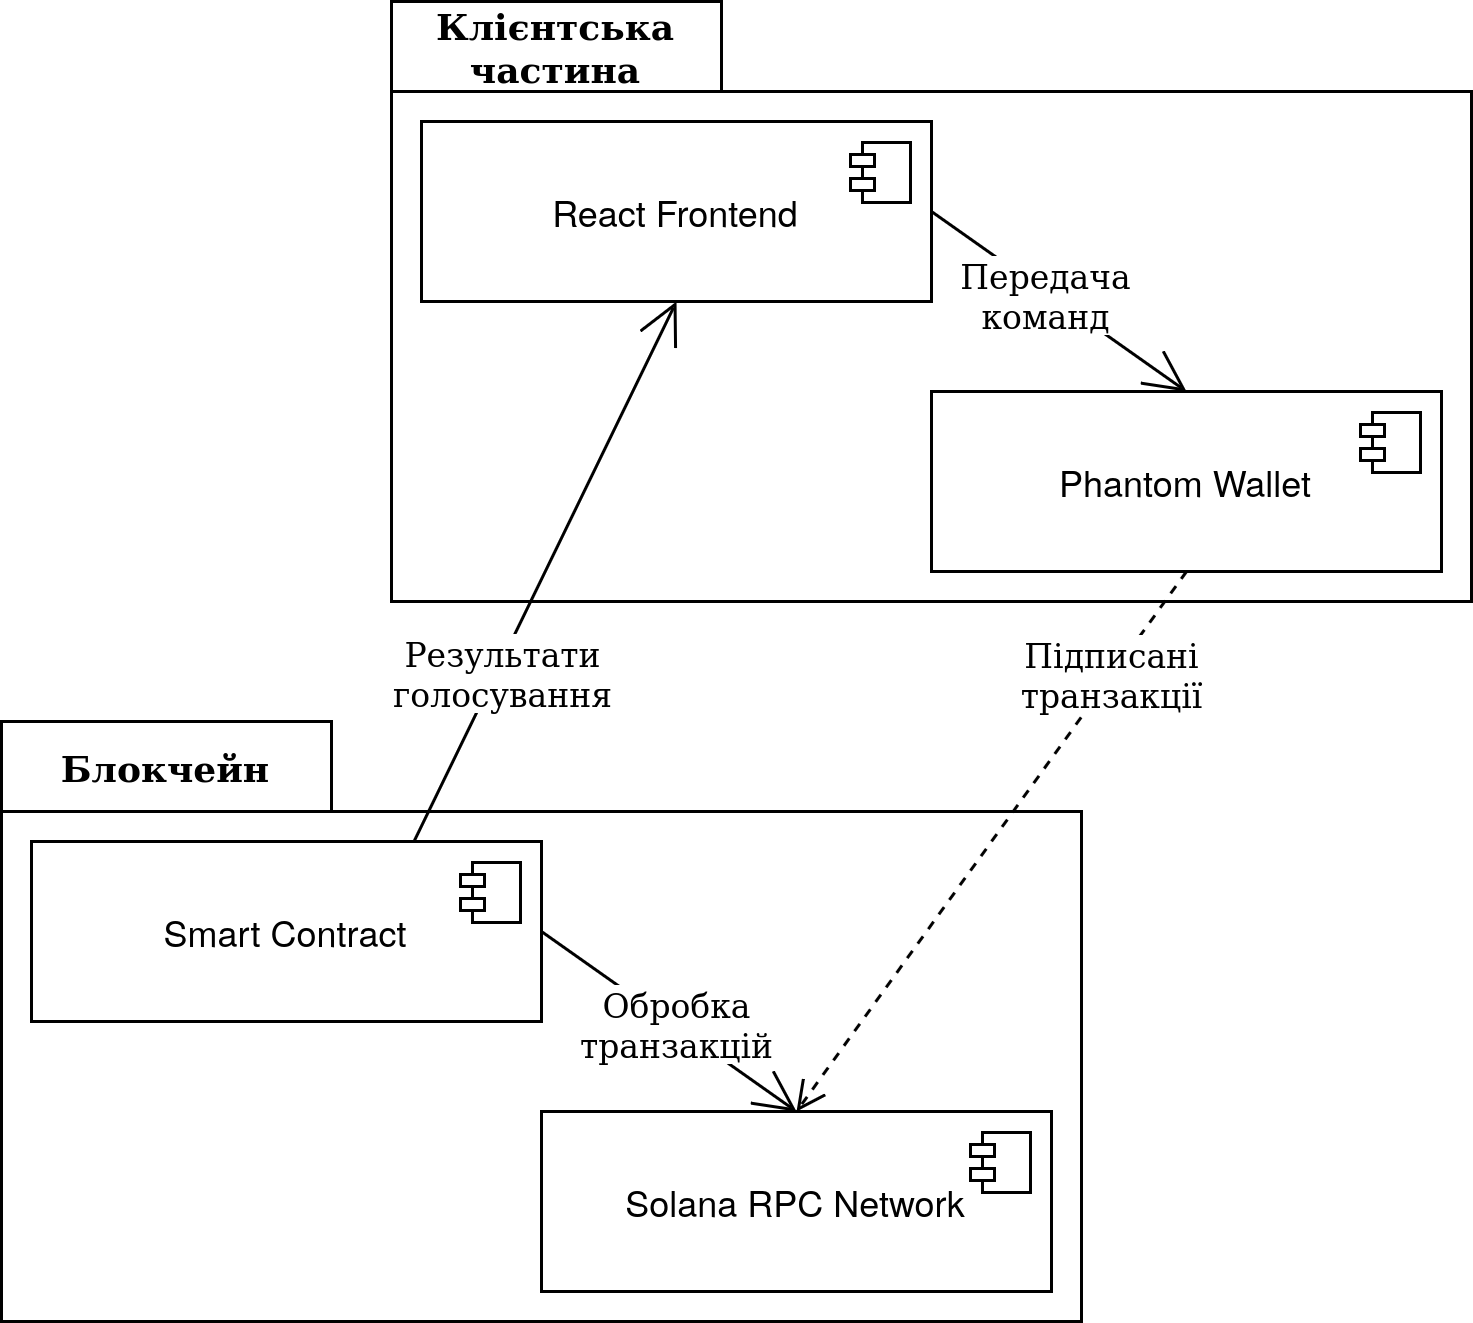
\includegraphics[scale=0.31]{UMLComponent}
    \caption{Діаграма компонентів}
  \end{figure}
  
  \chapter{Діаграма прецедентів}
  \label{app:UMLUseCase}
  
  \begin{figure}[H]
    \centering
    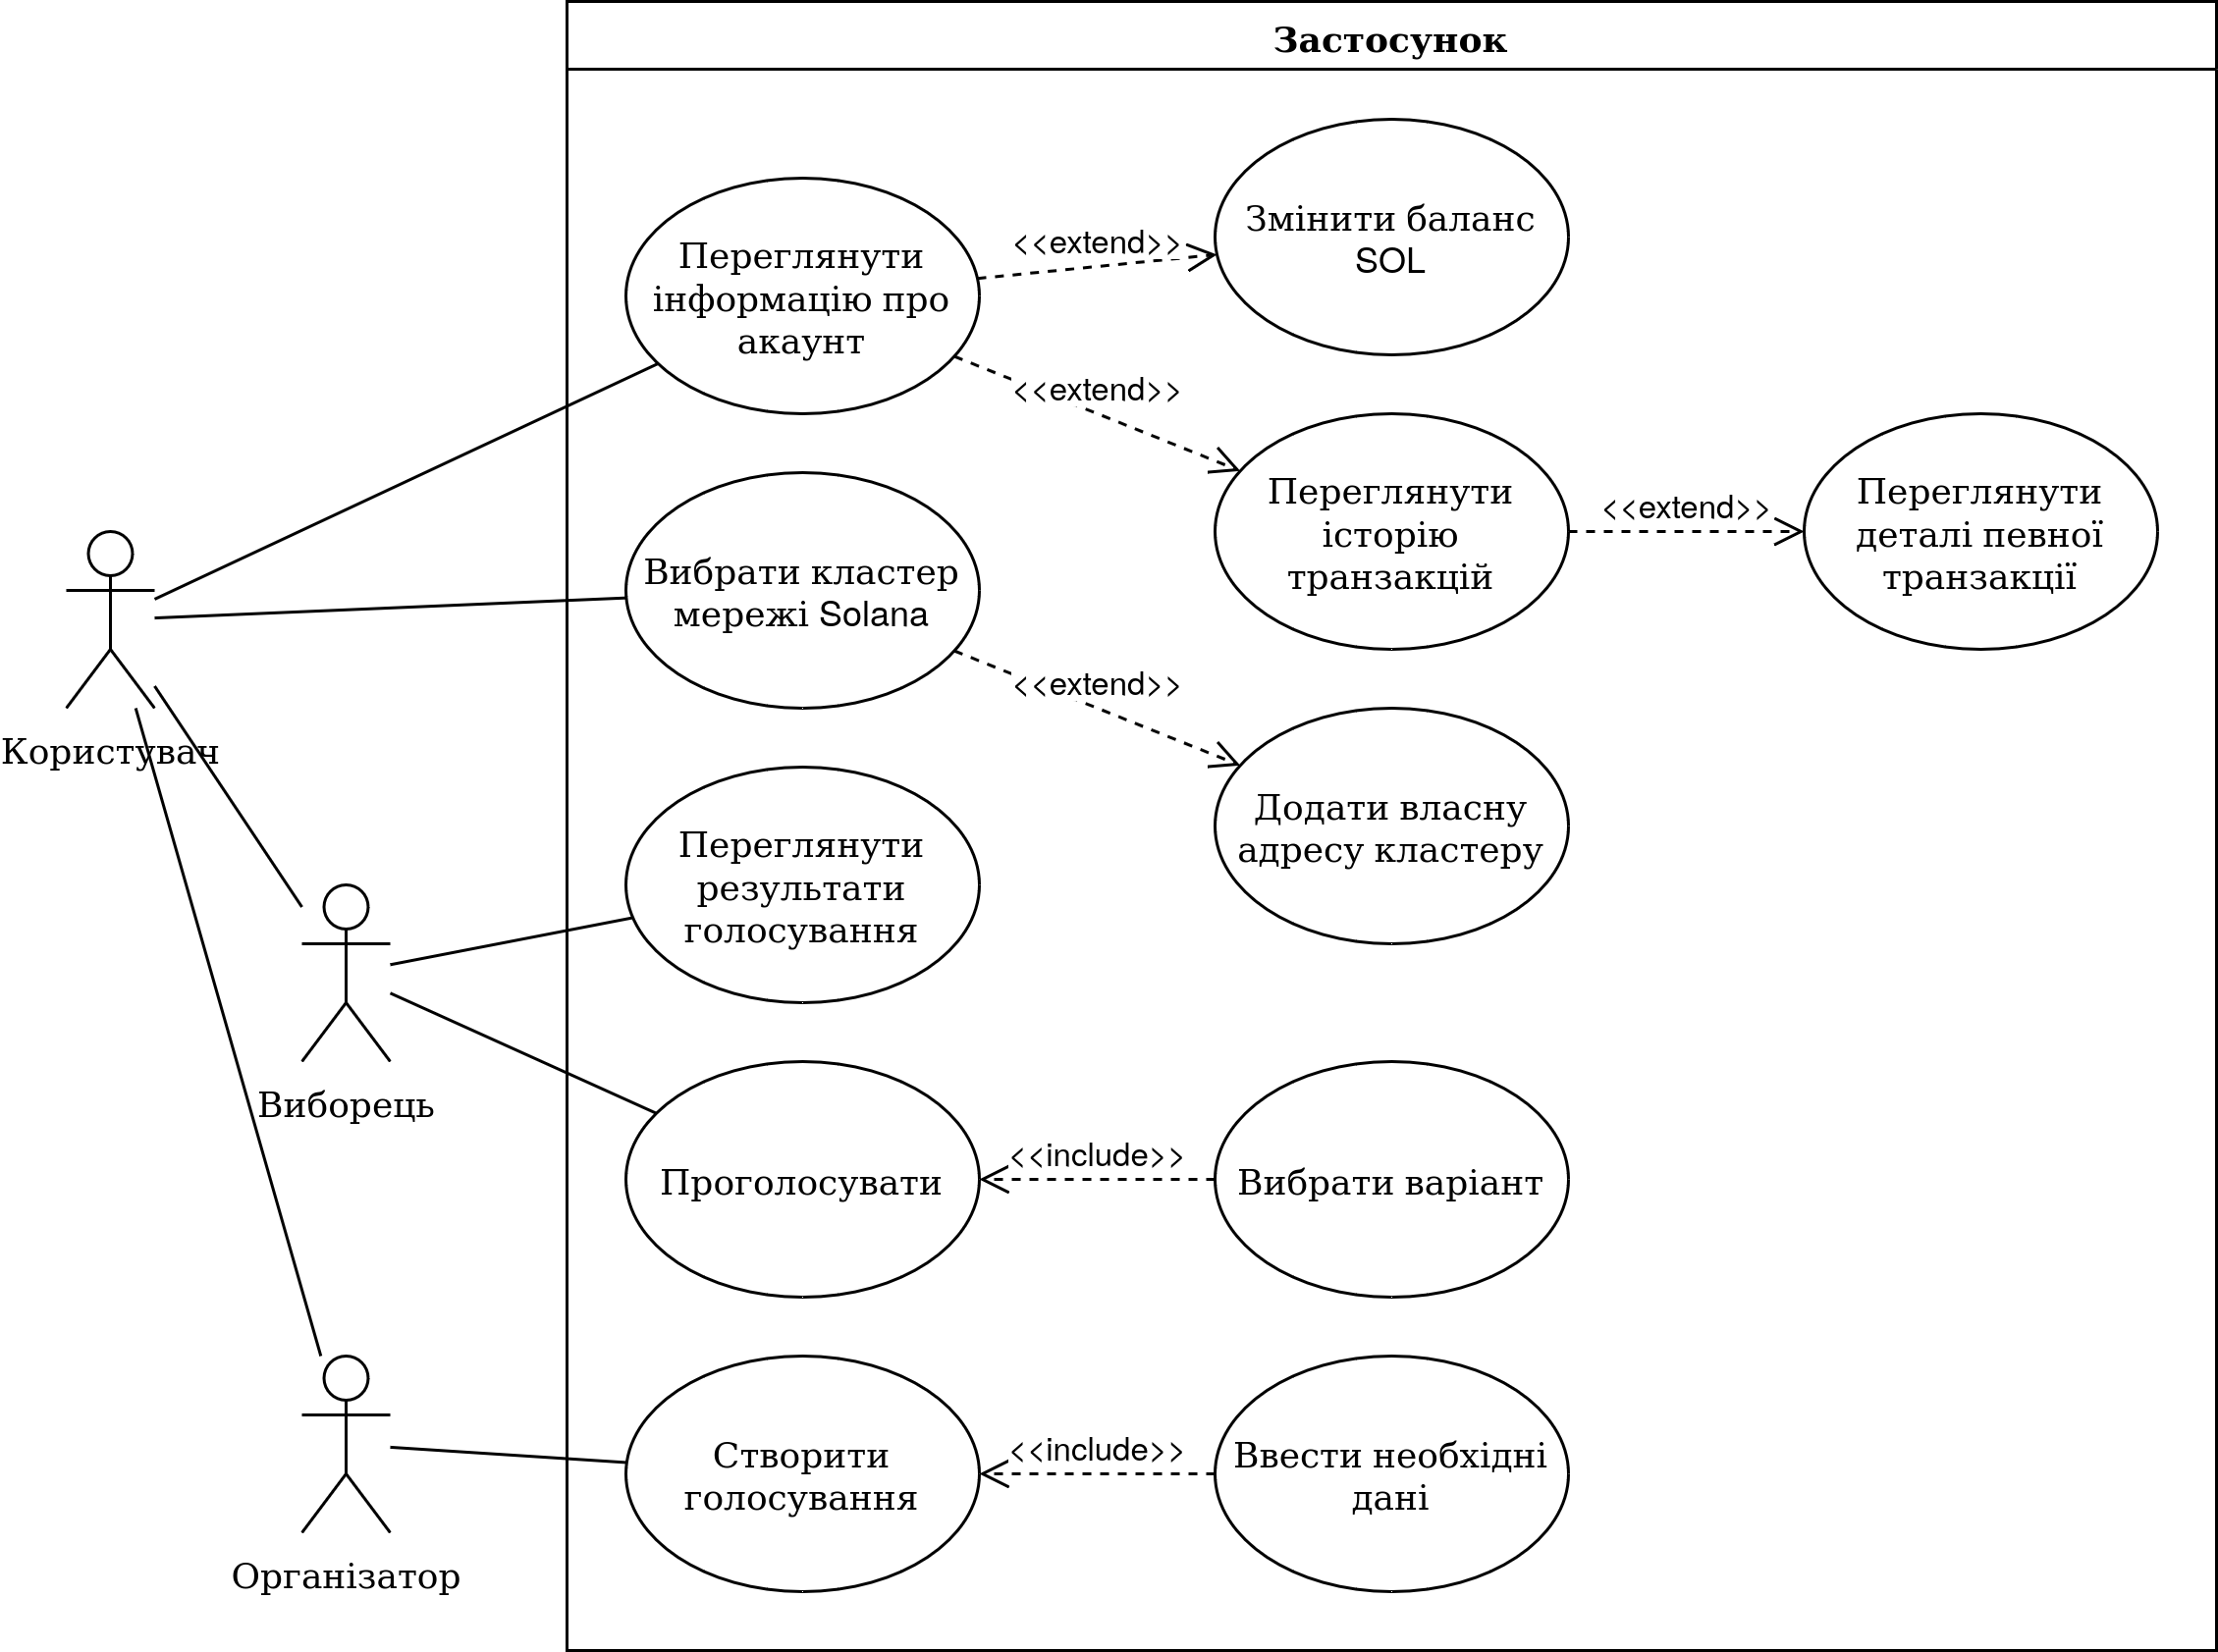
\includegraphics[scale=0.21]{UMLUseCase}
    \caption{Діаграма прецедентів}
  \end{figure}
  
  \chapter{Приклад інтерфейсу користувача}
  \label{app:UI}
  
  \begin{figure}[H]
    \centering
    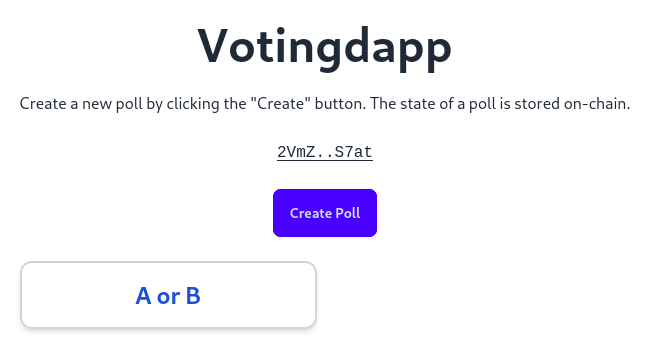
\includegraphics[scale=0.5]{UIPolls}
    \caption{Перегляд списку голосувань}
  \end{figure}
  
  \begin{figure}[H]
    \centering
    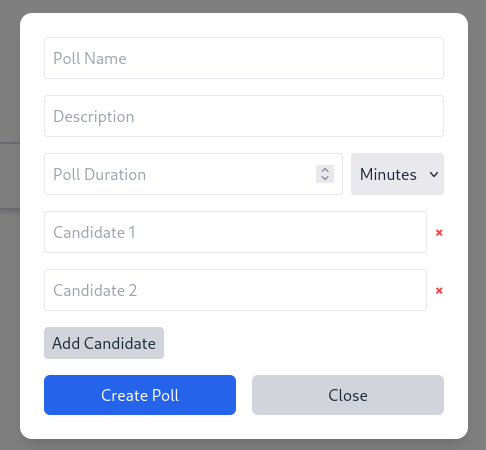
\includegraphics[scale=0.5]{UICreate}
    \caption{Форма для створення голосування}
  \end{figure}
  
  \begin{figure}[H]
    \centering
    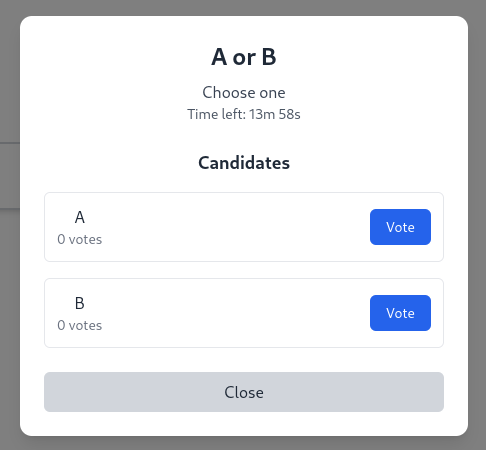
\includegraphics[scale=0.5]{UIVote}
    \caption{Форма для подачі голосу}
  \end{figure}
  
  \begin{figure}[H]
    \centering
    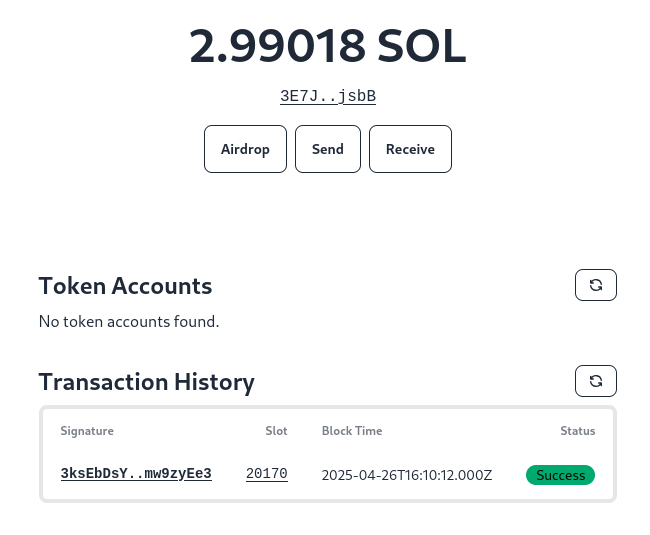
\includegraphics[scale=0.5]{UIAccount}
    \caption{Відображення інформації про баланс акаунту та історії транзакцій}
  \end{figure}
  
  \begin{figure}[H]
    \centering
    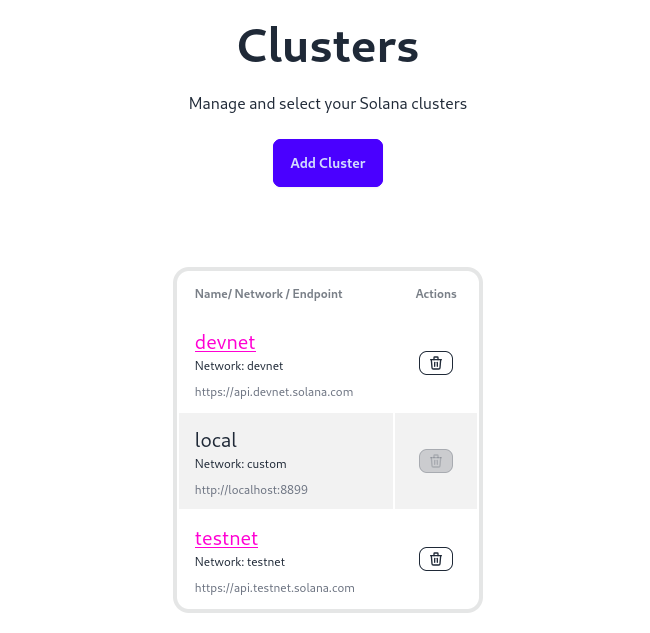
\includegraphics[scale=0.5]{UIClusters}
    \caption{Сторінка зі списком кластерів мережі}
  \end{figure}
  
\end{document}